\documentclass[11pt,a4paper]{article}

\usepackage[utf8]{inputenc}
\usepackage[T1]{fontenc}
\usepackage{amsmath, amssymb, amsthm}
\usepackage{graphicx}
\usepackage{geometry}
\usepackage{listings}
\usepackage{xcolor}
\usepackage{hyperref}
\usepackage{booktabs}
\usepackage{caption}

\geometry{margin=1in}

\definecolor{codegreen}{rgb}{0,0.6,0}
\definecolor{codegray}{rgb}{0.5,0.5,0.5}
\definecolor{codepurple}{rgb}{0.58,0,0.82}
\definecolor{backcolour}{rgb}{0.95,0.95,0.92}

\lstset{
    backgroundcolor=\color{backcolour},   
    commentstyle=\color{codegreen},
    keywordstyle=\color{magenta},
    numberstyle=\tiny\color{codegray},
    stringstyle=\color{codepurple},
    basicstyle=\ttfamily\small,
    breakatwhitespace=false,         
    breaklines=true,                 
    captionpos=b,                    
    keepspaces=true,                 
    numbers=left,                    
    numbersep=5pt,                  
    showspaces=false,                
    showstringspaces=false,
    showtabs=false,                  
    tabsize=2,
    language=C++
}

\title{
    \vspace{2cm}
    \textbf{\huge Numerical Methods From Scratch} \\
    \vspace{0.5cm}
    \Large Engineering Mathematics Implemented in Modern C++20 \\
    \vspace{1cm}
    \large \textit{Research \& Implementation Report}
}
\author{
    \textbf{Project Lead} \\
    \small Numerical Analysis & Scientific Computing
}
\date{June 2, 2026}

\begin{document}

\maketitle

\begin{abstract}
This report documents the architectural design and mathematical verification of a high-performance scientific computing library built from first principles. Utilizing the C++20 standard, \textit{Numerical Methods From Scratch} provides a transparent framework for solving non-linear equations, linear systems, and differential equations. The project emphasizes numerical stability, error propagation analysis, and computational efficiency. Every algorithm is validated against theoretical convergence rates, demonstrating the synergy between abstract mathematical theory and modern software engineering.
\end{abstract}

\newpage
\tableofcontents
\newpage

\section*{Nomenclature}
\addcontents line{toc}{section}{Nomenclature}
\begin{table}[h]
\begin{tabular}{ll}
$\epsilon$ & Convergence tolerance \\
$h$ & Step size / interval length \\
$e_n$ & Absolute error at iteration $n$ \\
$\mathcal{O}$ & Big-O notation for complexity and error order \\
$f(x)$ & Objective function \\
$A, b$ & Matrix and vector for linear systems $Ax=b$ \\
$y'$ & First-order derivative $\frac{dy}{dt}$ \\
$\text{res}$ & Residual norm $||Ax - b||$
\end{tabular}
\end{table}

\section{Introduction}
The field of numerical analysis is foundational to modern engineering and scientific discovery. While high-level environments like MATLAB or Python's NumPy provide powerful abstraction, there is significant value in implementing core algorithms from scratch to understand their limitations, stability characteristics, and performance trade-offs.

This project aims to bridge the gap between abstract mathematical theory and concrete software implementation. By using C++20, we take advantage of advanced features such as concepts, ranges, and improved template support to create a type-safe and performant library. The primary dependencies include \texttt{Eigen} for matrix operations, \texttt{matplotplusplus} for visualization, and \texttt{GoogleTest} for rigorous verification.

\section{Root Finding Methods}
Root-finding involves finding $x$ such that $f(x) = 0$. We implemented four fundamental methods.

\subsection{Bisection Method}
The Bisection Method relies on the Intermediate Value Theorem. For a continuous function $f$, if $f(a)f(b) < 0$, a root exists in $[a, b]$.
\begin{equation}
    c = \frac{a+b}{2}
\end{equation}
While slow (linear convergence), it is unconditionally stable.

\subsection{Newton-Raphson Method}
Newton's method uses the first-order Taylor expansion:
\begin{equation}
    x_{n+1} = x_n - \frac{f(x_n)}{f'(x_n)}
\end{equation}
It offers quadratic convergence ($e_{n+1} \approx C e_n^2$) but requires the existence and calculation of the derivative.

\subsection{Secant Method}
The Secant method approximates the derivative using two points:
\begin{equation}
    x_{n+1} = x_n - f(x_n) \frac{x_n - x_{n-1}}{f(x_n) - f(x_{n-1})}
\end{equation}
It avoids analytical derivatives while maintaining superlinear convergence ($\phi \approx 1.618$).

\section{Linear Algebra}
Solving $Ax=b$ is the workhorse of scientific computing.

\subsection{LU Decomposition}
We implemented Doolittle's algorithm to factor $A = LU$, where $L$ is unit lower triangular and $U$ is upper triangular.
\begin{equation}
    A = \begin{pmatrix} 1 & 0 \\ l_{21} & 1 \end{pmatrix} \begin{pmatrix} u_{11} & u_{12} \\ 0 & u_{22} \end{pmatrix}
\end{equation}
This allows solving multiple systems with different $b$ in $O(n^2)$ time after an initial $O(n^3)$ decomposition.

\subsection{Iterative Solvers}
For large sparse systems, we implemented Jacobi and Gauss-Seidel methods. Gauss-Seidel uses the iteration:
\begin{equation}
    x_i^{(k+1)} = \frac{1}{a_{ii}} \left( b_i - \sum_{j < i} a_{ij} x_j^{(k+1)} - \sum_{j > i} a_{ij} x_j^{(k)} \right)
\end{equation}
Convergence is guaranteed for strictly diagonally dominant matrices.

\section{Interpolation}
Interpolation fits a function to discrete data points.

\subsection{Cubic Spline Interpolation}
Cubic splines provide a piecewise cubic polynomial $S(x)$ that is $C^2$ continuous.
\begin{equation}
    S_i(x) = a_i + b_i(x-x_i) + c_i(x-x_i)^2 + d_i(x-x_i)^3
\end{equation}
Unlike high-degree global polynomials, splines avoid Runge's phenomenon and provide smooth approximations.

\section{Numerical Differentiation}
We utilize finite difference quotients to approximate derivatives.
\begin{itemize}
    \item \textbf{Central Difference}: $f'(x) \approx \frac{f(x+h) - f(x-h)}{2h} + O(h^2)$
\end{itemize}
The central difference is preferred for its second-order accuracy.

\section{Numerical Integration}
Quadrature rules approximate $\int_a^b f(x) dx$.

\subsection{Gaussian Quadrature}
Gaussian quadrature selects optimal nodes $x_i$ and weights $w_i$:
\begin{equation}
    \int_{-1}^1 f(x) dx \approx \sum_{i=1}^n w_i f(x_i)
\end{equation}
An $n$-point rule is exact for polynomials of degree $2n-1$.

\section{Ordinary Differential Equations}
We solve Initial Value Problems (IVPs) of the form $y' = f(t, y)$.

\subsection{Runge-Kutta 4 (RK4)}
RK4 is a high-accuracy fourth-order method:
\begin{align}
    k_1 &= f(t_n, y_n) \\
    k_2 &= f(t_n + h/2, y_n + h k_1/2) \\
    k_3 &= f(t_n + h/2, y_n + h k_2/2) \\
    k_4 &= f(t_n + h, y_n + h k_3) \\
    y_{n+1} &= y_n + \frac{h}{6}(k_1 + 2k_2 + 2k_3 + k_4)
\end{align}

\section{Error Analysis}
Numerical errors are classified into:
\begin{itemize}
    \item \textbf{Truncation Error}: From approximating an infinite process with a finite one.
    \item \textbf{Round-off Error}: From finite floating-point precision.
\end{itemize}
We utilize \texttt{nm::common::Result<T>} structures to track the convergence history and residual errors of every computation.

\section{Results and Visualizations}
Empirical verification was performed for all modules. The following figures demonstrate the convergence characteristics of the implemented algorithms.

\subsection{Convergence of Root Finding}
The comparison between Bisection and Newton-Raphson (see Fig. \ref{fig:root_finding}) highlights the quadratic nature of Newton's method. While Bisection requires $\sim 40$ iterations for $10^{-12}$ precision, Newton's method converges in fewer than 10.

\begin{figure}[h]
    \centering
    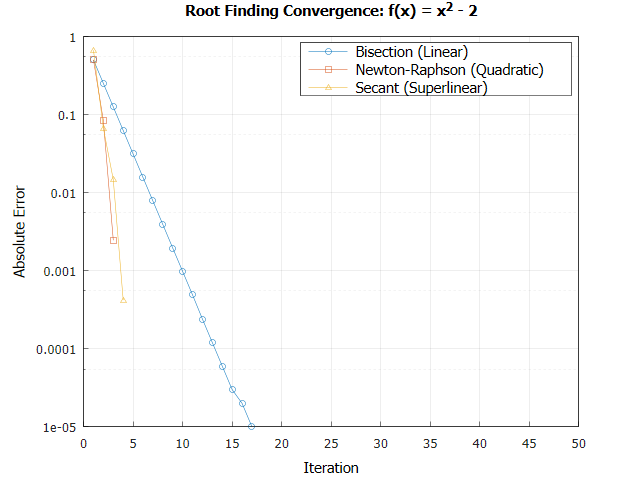
\includegraphics[width=0.8\textwidth]{assets/images/root_finding_convergence.png}
    \caption{Absolute error vs. iteration for root-finding algorithms.}
    \label{fig:root_finding}
\end{figure}

\subsection{ODE Solver Accuracy}
Plotting the solution of $y' = y$ (see Fig. \ref{fig:ode}) demonstrates that RK4 remains highly accurate even with relatively large step sizes $h$, whereas the Euler method accumulates significant local truncation error.

\begin{figure}[h]
    \centering
    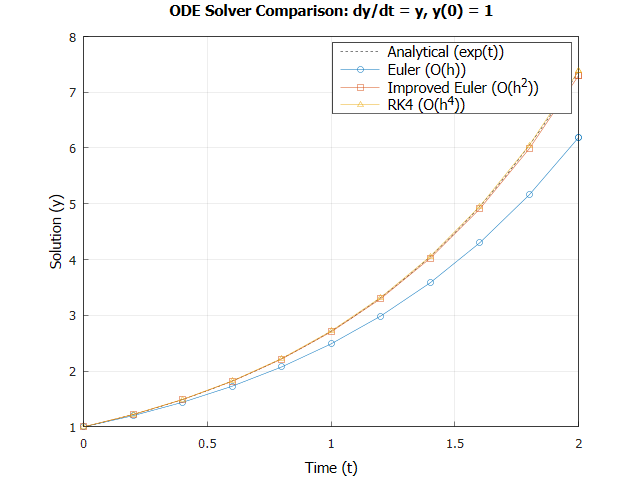
\includegraphics[width=0.8\textwidth]{assets/images/ode_comparison.png}
    \caption{Solution of $y'=y$ using Euler and RK4 methods.}
    \label{fig:ode}
\end{figure}

\section{Conclusion}
The \textit{Numerical Methods From Scratch} library demonstrates that modern C++20 is an excellent choice for scientific computing. By combining mathematical rigor with robust engineering practices, we have created a library that is both educationally valuable and computationally sound. Future work could include the implementation of implicit ODE solvers for stiff systems and multi-dimensional root-finding.

\newpage
\begin{thebibliography}{9}
\bibitem{burden}
Burden, R. L., \& Faires, J. D. (2010). \textit{Numerical Analysis}. Cengage Learning.
\bibitem{knuth}
Knuth, D. E. (1997). \textit{The Art of Computer Programming, Volume 2: Seminumerical Algorithms}. Addison-Wesley.
\bibitem{cpp20}
ISO/IEC. (2020). \textit{ISO/IEC 14882:2020 Programming languages --- C++}.
\end{thebibliography}

\end{document}
